\chapter{Pointers, references and function parameters}

\section{Pointers}

Declaring a variable means reserving a memory area, including several locations.
The number of locations depends on the type of the variable. For example, an
\texttt{int} variable occupies 4 bytes, a \texttt{float} variable occupies 4
bytes, and a \texttt{double} variable occupies 8 bytes. \\

Each memory location has a physicall address, which is a number that identifies
it. The address of a variable can be obtained by using the \texttt{\&} operator.
For example, the following code prints the address of the variable \texttt{a}:

\begin{lstlisting}[language=C++]
#include <iostream>
using namespace std;

int main() {
    int a = 10;
    cout << &a << endl;
    return 0;
}

// Output: 0x7fffbf7b3b7c (a mem address, it may vary)
\end{lstlisting}

The \texttt{\&} operator is called the \textbf{address-of operator}.\\

A pointer is a variable that stores the address of another variable. The type of
the pointer must be the same as the type of the variable whose address it will
store. For example, the following code declares a pointer to an integer variable
and assigns the address of the variable \texttt{a} to it:

\begin{lstlisting}[language=C++]
#include <iostream>
using namespace std;

int main() {
    int a = 10;
    int *p = &a;
    cout << p << endl;
    cout << *p << endl;
    return 0;
}

// Output: 
0x7fffbf7b3b7c (a mem address, it may vary)
10
\end{lstlisting}


The \texttt{*} operator is called the \textbf{dereference operator}. It is used
to access the value stored in the memory location pointed by the pointer. In the
example above, \texttt{*p} is equivalent to \texttt{a}. Note that the operator is
used to declare a pointer, but it is also used to access the value stored in the
memory location pointed by the pointer. This is a common source of confusion.\\

The following code shows how to declare a pointer to a \texttt{float} variable:

\begin{lstlisting}[language=C++]
#include <iostream>
using namespace std;

int main() {
    float b = 3.14;
    float *q = &b;
    cout << q << endl;
    cout << *q << endl;
    return 0;
}

// Output:
0x7fffbf7b3b7c (a mem address, it may vary)
3.14
\end{lstlisting}

As you can see, the code is very similar to the previous example. The only
difference is that the type of the pointer is \texttt{float *} instead of
\texttt{int *}. Pointers can store the address of any variable, regardless of its
type, but the type of the pointer must match the type of the variable whose
address it will store.

\subsection{Pointers to pointers}

There are no limits to how many type modifiers can be applied to a declarator.
When there is more than one modifier, they combine in ways that are logical, but
not always obvious. The \textbf{dereference operator} is a type modifier when 
it is used in a declaration. As such, it can be used multiple times.\\

A pointer is an object in memory, so like any other object, it has an address.
Therefore, we can store the address of a pointer on another pointer. For this,
we use two dereferencing operators \texttt{**}. There is no limit to how many 
of \texttt{*} we can stack, and each one will refer to a new pointer level.\\

\begin{lstlisting}[language=C++]
int val = 1024;
int *pi = &ival;
int **ppi = &pi;

cout << "direct value: " << val << "\n";
cout << "indirect value: " << *pi << "\n";
cout << "double indirect value: " << **ppi << "\n" << endl;

// Output
// direct value: 1024
// indirect value: 1024
// double indirect value: 1024
\end{lstlisting}

\section{Function parameters}

The general form of a function is:

\begin{lstlisting}[language=C++]
// function declaration
return_type function_name(type1 parameter1, type2 parameter2, ...)

// function definition
return_type function_name(type1 parameter1, type2 parameter2, ...)
{
    // function body
}
\end{lstlisting}

In a function definition, we use formal parameters represeinting a symbolic
reference (identifier) to objects used within the function. The initial value of
formal parameters is defined when the function is called using the actual 
parameters specified by the caller. Let us see an example:\\

\begin{lstlisting}[language=C++]
#include <iostream>
using namespace std;

double circ(double radius) {
    double res;
    res = 2 * 3.1416 * radius;
    return res;
}

int main() {
    double r = 5.0;
    double c = circ(r);
    cout << c << endl;
    return 0;
}

// Output: 31.416
\end{lstlisting}

In the example above, the function \texttt{circ} calculates the circumference of
a circle given its radius. Here, \texttt{radius} is a formal parameter, while
\texttt{r} is an actual parameter. The function is called with the actual
parameter \texttt{r}, and the value of \texttt{r} is copied to the formal
parameter \texttt{radius}.\\

The exchange of information with the passing of parameters between the caller and callee
can take place in two ways:

\begin{itemize}
    \item \textbf{Passing by value}
    \item \textbf{Passing by reference}
\end{itemize}

\subsection{Passing by value}

When passing by value, the actual parameter is copied to the formal parameter.
This means that any changes made to the formal parameter do not affect the 
actual parameter. For example:\\

\begin{lstlisting}[language=C++]
#include <iostream>
using namespace std;

void swap(int x, int y) {
    int temp;
    temp = x;
    x = y;
    y = temp;
}

int main() {
    int a = 10, b = 20;
    swap(a, b);
    cout << a << " " << b << endl;
    return 0;
}

// Output: 10 20
\end{lstlisting}

In the example above, the function \texttt{swap} is supposed to swap the values
of the variables \texttt{x} and \texttt{y}. However, the function does not work
as expected because the parameters are passed by value. The function receives
copies of the actual parameters, so any changes made to the formal parameters do
not affect the actual parameters.

\subsection{Passing by reference}

When passing by reference, the address of the actual parameter is passed to the
formal parameter. This means that the formal parameter is an alias of the actual
parameter. In other words, the formal and the actual parameters refer to the same
memory location. Any changes made to the formal parameter affect the actual
parameter. For example:\\

\begin{lstlisting}[language=C++]
#include <iostream>
using namespace std;

void swap(int* x, int* y) {
    int temp;
    temp = *x;
    *x = *y;
    *y = temp;
}

int main() {
    int a = 10, b = 20;
    swap(&a, &b);
    cout << a << " " << b << endl;
    return 0;
}

// Output: 20 10
\end{lstlisting}

In the example above, the function \texttt{swap} receives the addresses of the
variables \texttt{x} and \texttt{y}. The function swaps the values of the
variables by dereferencing the pointers. The function works as expected because
the parameters are passed by reference.\\

An important observation: arrays are always passed by reference. This means that
any changes made to an array in a function affect the original array. This is 
because the name of an array is a pointer to the first element of the array. For
example:\\

\begin{lstlisting}[language=C++]
#include <iostream>
using namespace std;

void change(int* arr, int n) {
    for (int i = 0; i < n; i++) {
        arr[i] = arr[i] * 2;
    }
}

int main() {
    int arr[] = {1, 2, 3, 4, 5};
    int n = sizeof(arr) / sizeof(arr[0]);
    change(arr, n);
    for (int i = 0; i < n; i++) {
        cout << arr[i] << " ";
    }
    cout << endl;
    return 0;
}

// Output: 2 4 6 8 10
\end{lstlisting}

In the example above, the function \texttt{change} receives the address of the
array \texttt{arr} and the size of the array \texttt{n}. The function multiplies
each element of the array by 2. The function works as expected because the array
is passed by reference.

\subsection{Passing by value vs passing by reference}

When you pass by value:

\begin{itemize}
    \item The actual parameter is copied to the formal parameter.
    \item It requires a lot of time to perform the copy if the parameter is large.
    \item Actual parameters and formal parameters are different.
    \item You cannot return a value to the caller without a return statement.
\end{itemize}

When you pass by reference:

\begin{itemize}
    \item The address of the actual parameter is passed to the formal parameter.
    \item It requires less time to pass the address than to copy the parameter,
    since the address has a fixed size.
    \item Actual parameters and formal parameters are the same.
    \item You can return a value to the caller by changing the value of the
    formal parameter.
\end{itemize}

\section{References}

A reference is an alias for a variable. It is a constant pointer that is
automatically dereferenced. A reference is declared by using the \texttt{\&}
operator. It must be always initialized when declared, and it cannot be changed
after initialization. For example:\\

\begin{lstlisting}[language=C++]
#include <iostream>
using namespace std;

int main() {
    int a = 10;
    int &b = a;
    cout << a << " " << b << endl;
    b = 20;
    cout << a << " " << b << endl;
}

// Output:
10 10
20 20
\end{lstlisting}

In the example above, the reference \texttt{b} is an alias for the variable
\texttt{a}. This means that \texttt{b} and \texttt{a} refer to the same memory
location. Any changes made to \texttt{b} affect \texttt{a}, and vice versa.\\

When we initialize a variable, the value of the inititializer is copied into
the object we are creating. When we define a reference, instead of copying
the initializer value, we bind the reference to its initializer. Once initialized,
a reference cannot be reseated to refer to a different object, and that is why
references must be initialized when declared. This is what we call a non-assignable
type.\\

When we fetch the value of a reference, we are actually fetching the value of
the object to which the reference is bound. When we use a reference as an
initializer, we are actually using the value of the object to which the reference
is bound. For example:\\

\begin{lstlisting}[language=C++]
int i = 7;
int &r = i; // r is a reference to i
int &r2 = r; // r2 is a reference to the object to which r is bound
int j = r; // j is initialized by the value in i
\end{lstlisting}

\subsection{References vs pointers}

References and pointers are similar in that they both provide an alternative way
to access an object. However, there are some differences between them:

\begin{itemize}
    \item A pointer is a compound type that holds a memory address. A reference
    just is an alias for an already existing object.
    \item Like references, pointers can be used for indirect access to an object.
    \item Unlike a reference, a pointer is an object that has its own address and
    can be assigned and copied to other pointers. A single pointer can point to
    different objects during its lifetime.
    \item Like other built-in types, pointers have undefined values if they are
    not initialized, so we have to be careful when using them.
    \item A reference is an alias for an object, and once a reference is initialized,
    it cannot be made to refer to a different object. A reference must be initialized
    when it is defined.
\end{itemize}

Note that the operators \texttt{*} and \texttt{\&} are used as both an operator in an
expression and as part of a declaration. The context in which the operator is used
determines what the symbol means.

\subsection{References as function parameters}

\texttt{C++} relies on references to implement pass by reference mechanism. This
simplifies the syntax for the caller and the callee. When a reference is passed
to a function, the function receives an alias to the actual parameter. This means
that any changes made to the formal parameter affect the actual parameter.\\

Let us see an example:\\

\begin{lstlisting}[language=C++]
#include <iostream>
using namespace std;

void swap(int &x, int &y) {
    int temp;
    temp = x;
    x = y;
    y = temp;
}

int main() {
    int a = 10, b = 20;
    swap(a, b);
    cout << a << " " << b << endl;
    return 0;
}

// Output: 20 10
\end{lstlisting}

In the example above, the function \texttt{swap} receives references to the
variables \texttt{x} and \texttt{y}. The function swaps the values of the
variables. The function works as expected because the parameters are passed by
reference.

\subsection{\texttt{const} references}

We might want to define a variable whose value cannot be changed, for example,
to refer to the size of a buffer. We can make a variable unchangeable by using
the \texttt{const} keyword. For example:\\

\begin{lstlisting}[language=C++]
const int bufSize = 512;
bufSize = 512; // error: cannot assign to a const object
\end{lstlisting}

Since we can't change the value of a \texttt{const} object, it must be always
initialized when declared, i.e., this is also a non-assignable type. 
By default, \texttt{const} objects are local to the
file in which they are defined. When a \texttt{const} object is initialized from 
a compile-time constant, our compiler will usually substitute the uses of the 
variable with the value of the constant during compilation.\\

We can also define a reference to a \texttt{const} object. To do so, we use a 
reference to \texttt{const} type. Unlike an ordinary reference, a reference to
\texttt{const} cannot be used to change the value of the object to which it is
bound.\\

This is useful when we want to pass an argument to a function by reference, 
but we don't want the function to change the value of the argument. In other
words, \texttt{const} references can be used to pass large objects to functions
in read-only mode, obtaining the benefits of pass by reference without the risk
of changing the value of the object.\\

Let us see an example:\\

\begin{lstlisting}[language=C++]
#include <iostream>
using namespace std;

double circ(const double &radius) {
    double res;
    res = 2 * 3.1416 * radius;
    //radius = 10;  --> f we try to change the value of radius, we get an error 
    return res;
}

int main() {
    double r = 5.0;
    double c = circ(r);
    cout << c << endl;
    return 0;
}

// Output: 31.416
\end{lstlisting}

In the example above, the function \texttt{circ} receives a reference to a
\texttt{const} variable. The function calculates the circumference of a circle
given its radius. In this case, we protect the value of the radius from being
changed by using a reference to a \texttt{const} variable.\\

An important thing we need to notice is that the reference to \texttt{const}
restricts only what we can do through that reference. Binding a reference to
\texttt{const} to an object says nothing about whether the underlying object 
itself is \texttt{const}, and because of this, it might be changed by other means:\\

\begin{lstlisting}[language=C++]
int i = 42;
int &r1 = i;
const int &r2 = i;

r1 = 0; // r1 is not const, so i is now 0
r2 = 0; // error: r2 is a reference to const
\end{lstlisting}

\section{Guidelines for passing parameters}

When passing parameters to a function, we have to decide whether to pass by
value, by reference, or by \texttt{const} reference. Here are some guidelines:

\begin{itemize}
    \item If the parameter is small and we don't want the function to change its
    value, we can pass by value.
    \item If the parameter is large and we don't want the function to change its
    value, we can pass by \texttt{const} reference.
    \item If the parameter is large and we want the function to change its value,
    we can pass by reference.
\end{itemize}

In other words:

\begin{itemize}
    \item Use call-by-value for very small objects (base types).
    \item Use call-by-const-reference for large objects.
    \item Use call-by-reference only when you must return a result,
    rather than modify an object through a reference argument.
\end{itemize}

\section{Variables scope}

The scope of an identifier (to a variable, a function, etc) is the region of the program in which the identifier
can be referenced. Some identifiers can be referenced throughout the program, while others can only be referenced
within a specific portion of the program. For example, when we declare a local variable in a block (e.g., in a for loop),
it can be referenced only in that block or blocks nested within it.

\subsection{Methods of variable creation}

There are three methods of creating variables in \texttt{C++}:

\subsubsection{Global variables}

Global variables are declared outside of all functions. They can be referenced throughout the whole program. They are
stored in the static data. For example:\\

\begin{lstlisting}[language=C++]
#include <iostream>
using namespace std;

int x = 10; // global variable (bad practice)

int main() {
    cout << x << endl;
    return 0;
}

// Output: 10
\end{lstlisting}

These variables are difficult to debug and maintain, so in general, it is considered a bad practice to use them.
However, global constants are an exception to this rule. For example:\\

\begin{lstlisting}[language=C++]
#include <iostream>
using namespace std;

const double PI = 3.1416; // global constant

int main() {
    cout << PI << endl;
    return 0;
}

// Output: 3.1416
\end{lstlisting}

In this case, the global constant \texttt{PI} is used to store the value of $\pi$. This is an accepted practice because
the value of $\pi$ is constant and will not change throughout the program, and will probably be used in many parts 
of the program.

\subsubsection{Local on the fly variables}

This type of variables are simply created right when they are needed. They are only available within the block in which
they were created, and are stored in the stack. For example:\\

\begin{lstlisting}[language=C++]
#include <iostream>
using namespace std;

int main() {
    for (int i = 0; i < 5; i++) { // i is a local on the fly variable
        cout << i << " ";
    }
}

// Output: 0 1 2 3 4
\end{lstlisting}

\subsubsection{Local defined variables}

These variables are created at the beginning of the block in which they are defined, and are available throughout the block.
They are stored in the stack. This is the most common way of creating variables. For example:\\

\begin{lstlisting}[language=C++]
#include <iostream>
using namespace std;

int main() {
    int x = 10; // local defined variable
    cout << x << endl;
    return 0;
}

// Output: 10
\end{lstlisting}

\subsection{Global and local declarations}

When a local variable has the same name as a global variable, the local variable takes precedence. For example:

\begin{lstlisting}[language=C++]
#include <iostream>
using namespace std;

int x = 10; // global variable

int main() {
    int x = 20; // local variable
    cout << x << endl;
    return 0;
}

// Output: 20
\end{lstlisting}

In the example above, the local variable \texttt{x} takes precedence over the global variable \texttt{x}. Be aware
that function parameters are also local variables, so the same rule applies. For example:\\

\begin{lstlisting}[language=C++]
#include <iostream>
using namespace std;

int x = 10; // global variable

void f(int x) {
    cout << x << endl;
}

int main() {
    f(20); // local variable
    return 0;
}

// Output: 20
\end{lstlisting}

\subsection{Lifetime of variables}

The lifetime of a variable is the period during which the variable exists in memory. The lifetime of a global variable
is the entire execution of the program, while the lifetime of a local variable is the period during which the function is
executed. When you call a function, memory will be allocated for all local variables defined inside the function. When the
function returns, the memory will be deallocated.

\section{\texttt{auto} specifier and range-for loops}

It is not uncommon to want to store the value of an expression in a variable declaration.
But to declare the variable, we have to know the type of that expression. 
Since \texttt{C++ 11}, we can let the compiler figure out the type for us, using
the \texttt{auto} type specifier.\\

Unlike other type specifiers, such as \texttt{double} or \texttt{int}, that name a
specific type, \texttt{auto} tells the compiler to deduce the type from the initializer.
That means that a variable using \texttt{auto} as its type specifier must have an 
initializer. Let us see an example:\\

\begin{lstlisting}[language=C++]
auto item = val1 + val2;
// item will be initialized to the result type of val1 + val2
\end{lstlisting}

\subsection{Range-for loops}

A range-for loop is a very useful tool to iterate over a container of elements (e.g.,
an array or a vector). Its sytax is similar to the simple for loop, but the iterator
variable gets the value of each element in the container, instead of each position
index. For example:\\

\begin{lstlisting}[language=C++]
std::vector<int> v = {10, 20, 30};

for (int i: v) {
    std::cout << i << " ";
}
// Output: 10 20 30
\end{lstlisting}

Note that in this case, every element of \texttt{v} is copied into \texttt{i}.
Sometimes, we might want to avoid the copy of each element, since they could
be large. For that, we can use references as such:\\

\begin{lstlisting}[language=C++]
// Assume that v is a vector of Strings
for (string &s : v) {
    cout << s << "\n";
}
\end{lstlisting}

In this way, we avoid the copy of each element to the iteration variable. We might even
want to avoid modyfing any element of the vector inside the range-for loop. In that
case, we could use a reference to \texttt{const}, instead of just a reference.\\

Sometimes, we might not be sure of the type of the objects inside a certain vector,
but we still want to iterate over them. For that, we can use the \texttt{auto} specifier
in the same way as before:\\

\begin{lstlisting}[language=C++]
for (auto e : v) {cout << e << "\n"} // e is a copy of all v[i]

for (auto &e : v) {cout << e << "\n"} // no copy

for (const auto &e : v) {cout << e << "\n"} // unmodifiable
\end{lstlisting}

\section{Iterators}

Until now, we have been using subscripts (\texttt{[n]}) to access the elements of
a container. There is a more general mechanism, the \textbf{iterators}, that we can
use for the same purpose.\\

The STL library defines several kinds of containers, and all of them have iterators,
but only a few support the subscript operator. We can think of an iterator as a 
pointer to access any container. Using iterators instead of subscripts allows us to
change the container type without changing our code.\\

Like pointers, iterators give us indirect access to an object, and they have also
operations to move from one element to another.\\

Types that have iterators have also members to return those iterators. These are
\texttt{begin()} and \texttt{end()}. The first one returns an iterator that denotes the
first element of the container, if there is one, while the second one returns an 
iterator positioned "one past the end" of the associated container. Let us see
an example:\\

\begin{lstlisting}
std::vector<int> v = {1, 2, 3};

auto b = v.begin();
auto e = v.end();

// The type should be vector::iterator, but we let the compiler deduce it
\end{lstlisting}

If the container is empty, the iterators returned by both methods are equal,
they are both off-the-end iterators. Here is another example:\\

\begin{lstlisting}[language=C++]
string s("some string");

for (auto it = s.begin(); it != s.end() && !isspace(*it); ++it) {
    *it = toupper(*it);
}
\end{lstlisting}

\subsection{Standard container iterator operations}

These operations apply to all STL iterators:

\begin{figure}[H]
\centering
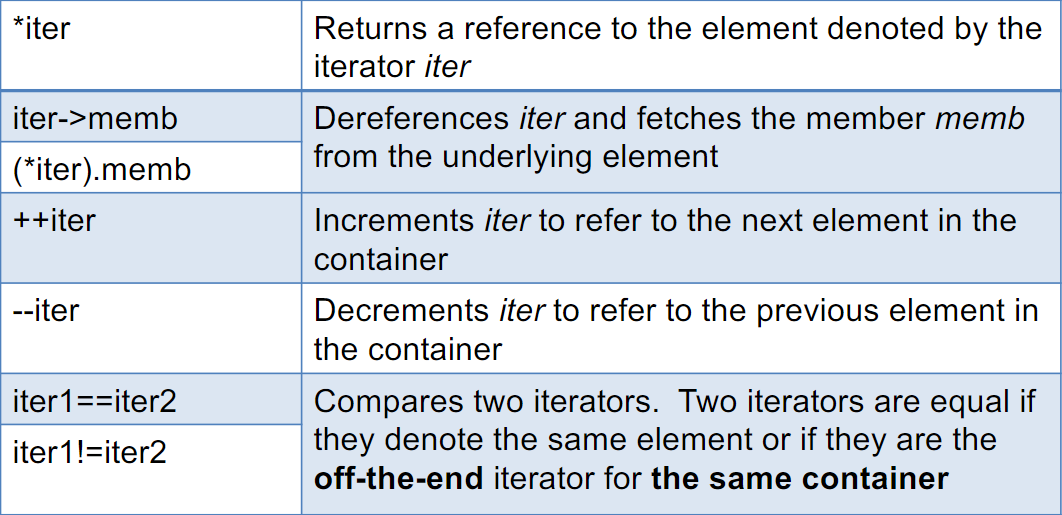
\includegraphics[width=0.7\textwidth]{figures/image_STL_it_op.png}
\caption{STL iterator operations}
\label{fig:STL_it_op}
\end{figure}

These operations apply only to vectors and strings:

\begin{figure}[H]
    \centering
    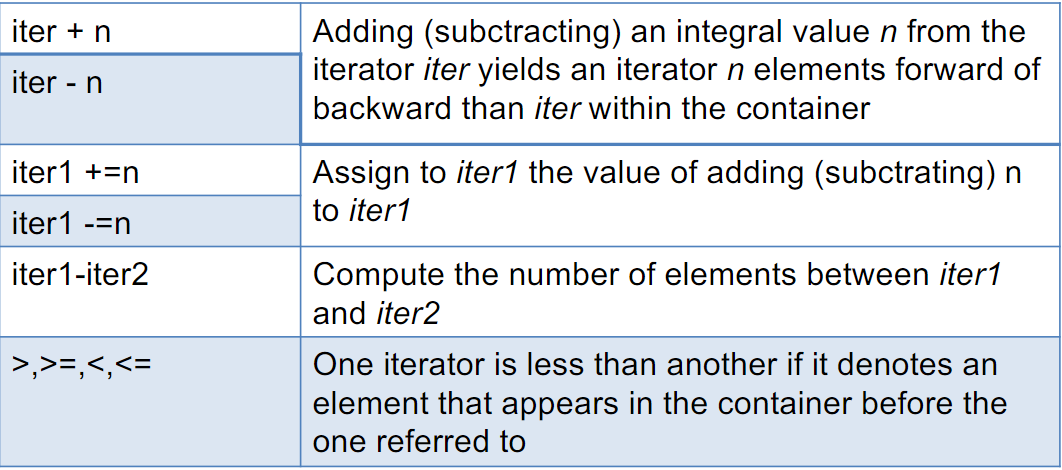
\includegraphics[width=0.7\textwidth]{figures/image_vec_str_it_op.png}
    \caption{Vector and String iterator operations}
    \label{fig:vec_str_it_op}
\end{figure}

\subsection{Constant iterators}

These type of iterators, called \texttt{const\_iterator}, are used when we 
need to read but not write to an object. To access these, the standard containers
have the methods \texttt{cbegin()} and \texttt{cend()}. They are used in the same
way as the other iterators, but the only constraint is that we cannot use them to
modify the elements inside the container.\\

\begin{lstlisting}[language=C++]
string s = "hello world";

for (auto it = s.cbegin(); it != s.cend(); ++it) {
    cout << *it;
}
\end{lstlisting}